\chapter{Datasets}

This thesis is based on 5 different already existing datasets.
This chapter discusses these datasets based on different criteria:

\begin{description}
    \item[source:] reference of the owner of the dataset and brief description of the original purpose of the dataset.
    \item[Patient sample:] statistics of the patients of whom medical images were collected such as age, gender and possible spine pathologies.
    \item[Technical information:] discusses the imaging technology, the image resolution and the spatial dimensions of the image. 
\end{description}

\section{Global overview of the different dataset}
\todo[inline]{Overview of the datasets gathered. MRI / CT, number of images, type of annotation}

\begin{SCtable}[\sidecaptionrelwidth][h]
 
    \begin{tabular}{ l l l l l} 
     \hline
     \hline
     Name & reference & imaging & Quantity & Annotation \\
          &           & technology & [images] & \\
     \hline 
    UWSpine & \cite{Glocker}  & \acrshort{ct} & 125 & point  \\ 
    xVertSeg & \cite{Yoa2015} & \acrshort{ct} & 15 & full \\
    UniSiegen  &  & \acrshort{mri} & 17 & full \\
    Zenobo & & \acrshort{mri} & 23 & semantic \\
    MyoSegmenTUM & S. Schlaeger & \acrshort{mri} &  54 & full \\
     \hline
     \hline
    \end{tabular}
    \caption{List of dataset references. For more details on the data quantity, please consult chapter \ref{seg:datasetcomparison}. 
    Notably the fact that some images were taken from the same patient is important. This means the dataset is grouped. 
    The agreement with prof. T. Vrtovec regarding the xVertSeg dataset can be found in appendix \ref{seg:datasetagreement}.}

\end{SCtable}

\begin{SCtable}[\sidecaptionrelwidth][h]
 
    \begin{tabular}{ l l l l} 
     \hline
     \hline
     Name & X & Y & Z \\
     \hline 
    UWSpine & Left-right & Anteroposterior & Craniocaudal \\
    xVertSeg & Left-right & Anteroposterior & Craniocaudal \\
    UniSiegen  &  Anteroposterior & Craniocaudal & Left-right \\
    Zenobo & Left-right & Anteroposterior & Craniocaudal (inverted) \\
    MyoSegmenTUM &  Anteroposterior & Craniocaudal & Left-right \\
     \hline
     \hline
    \end{tabular}
    \caption{List of dataset references. For more details on the data quantity, please consult chapter \ref{seg:datasetcomparison}. 
    Notably the fact that some images were taken from the same patient is important. This means the dataset is grouped. 
    The agreement with prof. T. Vrtovec regarding the xVertSeg dataset can be found in appendix \ref{seg:datasetagreement}.}

\end{SCtable}

\section{Comparison of the different datasets\label{seg:datasetcomparison}}

\subsection{xVertSeg}

The xVertSeg \cite{Ibragimov2012,Ibragimov2012} was kindly made available by prof. T. Vrtovec, see appendix \ref{seg:datasetagreement}.
This dataset contains 15 \acrshort{ct} scans of the lumbar spine. 
Full instance segmenation masks for all 5 lumbar vertebrae are present.
\todo[inline]{who did the segmentation}


\subsubsection{Patient statistics}

The patients in the xVertSeg dataset consist of 8 females and 7 males.
The age of these patients is slightly higher than for the other datasets.
The average patient in this dataset is 71 years old.
The age distribution between both genders is illustrated in figure \ref{fig:xVertSeg_Age}. 


\marginpar{
        % This file was created by tikzplotlib v0.9.8.
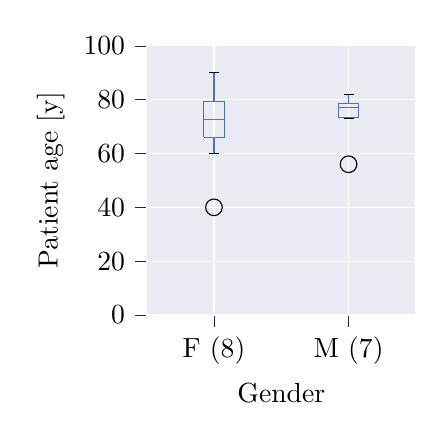
\begin{tikzpicture}

\definecolor{color0}{rgb}{0.917647058823529,0.917647058823529,0.949019607843137}
\definecolor{color1}{rgb}{0.298039215686275,0.447058823529412,0.690196078431373}
\definecolor{color2}{rgb}{0.768627450980392,0.305882352941176,0.32156862745098}

\begin{axis}[
axis background/.style={fill=color0},
axis line style={white},
height=5cm,
tick align=outside,
tick pos=left,
width=5cm,
x grid style={white},
xlabel={Gender},
xmajorgrids,
xmin=0.5, xmax=2.5,
xtick style={color=white!15!black},
xtick={1,2},
xticklabels={F (8),M (7)},
y grid style={white},
ylabel={Patient age [y]},
ymajorgrids,
ymin=0, ymax=100,
ytick style={color=white!15!black}
]
\addplot [color1, opacity=1]
table {%
0.925 66
1.075 66
1.075 79.25
0.925 79.25
0.925 66
};
\addplot [color1, opacity=1]
table {%
1 66
1 60
};
\addplot [color1, opacity=1]
table {%
1 79.25
1 90
};
\addplot [black, opacity=1]
table {%
0.9625 60
1.0375 60
};
\addplot [black, opacity=1]
table {%
0.9625 90
1.0375 90
};
\addplot [black, mark=o, mark size=3, mark options={solid,fill opacity=0}, only marks]
table {%
1 40
};
\addplot [color1, opacity=1]
table {%
1.925 73.5
2.075 73.5
2.075 78.5
1.925 78.5
1.925 73.5
};
\addplot [color1, opacity=1]
table {%
2 73.5
2 73
};
\addplot [color1, opacity=1]
table {%
2 78.5
2 82
};
\addplot [black, opacity=1]
table {%
1.9625 73
2.0375 73
};
\addplot [black, opacity=1]
table {%
1.9625 82
2.0375 82
};
\addplot [black, mark=o, mark size=3, mark options={solid,fill opacity=0}, only marks]
table {%
2 56
};
\addplot [color2, opacity=1]
table {%
0.925 72.5
1.075 72.5
};
\addplot [color2, opacity=1]
table {%
1.925 77
2.075 77
};
\end{axis}

\end{tikzpicture}

        \captionof{figure}{xVertSeg patients age distribution}
        \label{fig:xVertSeg_Age}
    }

\begin{SCtable}[\sidecaptionrelwidth][h]
    \centering
        \begin{tabular}{lrrrrrr}
\toprule
{} &  L1 &  L2 &  L3 &  L4 &  L5 &  Total \\
\midrule
biconcave &   6 &   7 &   8 &   4 &   2 &     27 \\
normal    &   5 &   6 &   4 &   4 &   7 &     26 \\
wedge     &   3 &   2 &   2 &   3 &   2 &     12 \\
crush     &   1 &   0 &   1 &   4 &   4 &     10 \\
\bottomrule
\end{tabular}

        \caption{All of the patients in the xVertSeg dataset suffer from spine pathologies.
        Most of these pathologies are identified as \textit{mild}.
        This table counts the spine pathologies and normal vertebrae observed over all 15 patients in the xVertSeg dataset.}
    
\end{SCtable}

\subsubsection{Technical information}

The xVertSeg dataset contains 15 \acrshort{ct} scans. 
These images 


\marginpar{
        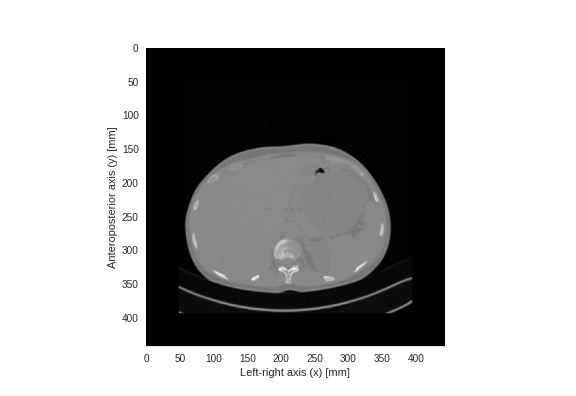
\includegraphics[width=5cm]{images/xVertSeg_image002_TransverseSlice.png}
        \captionof{figure}{Transverse slice: image002 of the xVertSeg dataset. }
        \label{fig:xVertSeg_Transverse}
    }

\marginpar{
        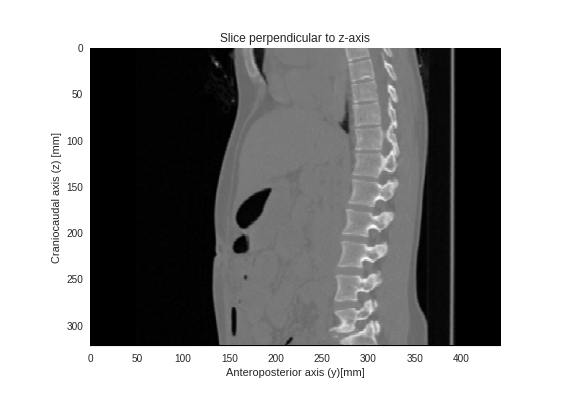
\includegraphics[width=5cm]{images/xVertSeg_image002_SagittalSlice.png}
        \captionof{figure}{Sagittal slice: image002 of the xVertSeg dataset. }
        \label{fig:xVertSeg_Sagittal}
    }

\begin{SCfigure}[][htb]
    \centering
    % This file was created by tikzplotlib v0.9.8.
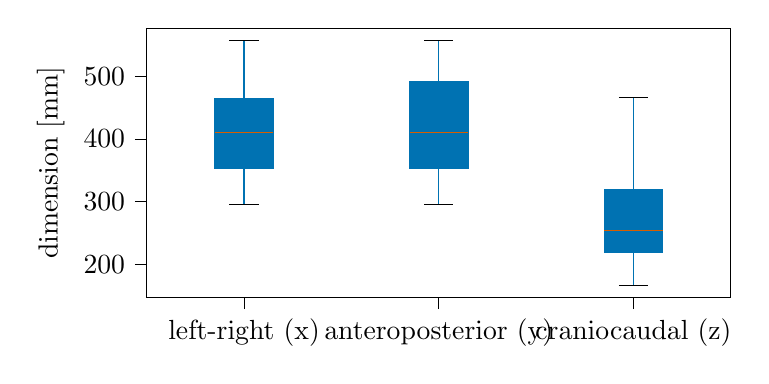
\begin{tikzpicture}

\definecolor{color0}{rgb}{0,0.447058823529412,0.698039215686274}
\definecolor{color1}{rgb}{0.835294117647059,0.368627450980392,0}

\begin{axis}[
height=5cm,
tick align=outside,
tick pos=left,
width=9cm,
x grid style={white!69.0196078431373!black},
xmin=0.5, xmax=3.5,
xtick style={color=black},
xtick={1,2,3},
xticklabels={left-right (x),anteroposterior (y),craniocaudal (z)},
y grid style={white!69.0196078431373!black},
ylabel={dimension [mm]},
ymin=147.344568, ymax=576.684072,
ytick style={color=black}
]
\addplot [color0, opacity=1]
table {%
1 352.99328
1 295.5264
};
\addplot [color0, opacity=1]
table {%
1 464.0768
1 557.16864
};
\addplot [black, opacity=1]
table {%
0.925 295.5264
1.075 295.5264
};
\addplot [black, opacity=1]
table {%
0.925 557.16864
1.075 557.16864
};
\addplot [color0, opacity=1]
table {%
2 352.99328
2 295.5264
};
\addplot [color0, opacity=1]
table {%
2 491.8562
2 557.16864
};
\addplot [black, opacity=1]
table {%
1.925 295.5264
2.075 295.5264
};
\addplot [black, opacity=1]
table {%
1.925 557.16864
2.075 557.16864
};
\addplot [color0, opacity=1]
table {%
3 219.777
3 166.86
};
\addplot [color0, opacity=1]
table {%
3 319.5245
3 466.3386
};
\addplot [black, opacity=1]
table {%
2.925 166.86
3.075 166.86
};
\addplot [black, opacity=1]
table {%
2.925 466.3386
3.075 466.3386
};
\path [draw=color0, fill=color0]
(axis cs:0.85,352.99328)
--(axis cs:1.15,352.99328)
--(axis cs:1.15,464.0768)
--(axis cs:0.85,464.0768)
--(axis cs:0.85,352.99328)
--cycle;
\path [draw=color0, fill=color0]
(axis cs:1.85,352.99328)
--(axis cs:2.15,352.99328)
--(axis cs:2.15,491.8562)
--(axis cs:1.85,491.8562)
--(axis cs:1.85,352.99328)
--cycle;
\path [draw=color0, fill=color0]
(axis cs:2.85,219.777)
--(axis cs:3.15,219.777)
--(axis cs:3.15,319.5245)
--(axis cs:2.85,319.5245)
--(axis cs:2.85,219.777)
--cycle;
\addplot [color1, opacity=1]
table {%
0.85 410.99776
1.15 410.99776
};
\addplot [color1, opacity=1]
table {%
1.85 410.99776
2.15 410.99776
};
\addplot [color1, opacity=1]
table {%
2.85 254.196
3.15 254.196
};
\end{axis}

\end{tikzpicture}

    \caption{Distribution of the dimensions of the xVertSeg images}
\end{SCfigure}


